\documentclass[10pt,a4paper]{article}
\usepackage[margin=17mm]{geometry}
\usepackage[T1]{fontenc}
\usepackage{lmodern,amsmath,amssymb,graphicx,booktabs,array,xcolor,hyperref}
\hypersetup{colorlinks=true,urlcolor=blue,pdftitle={Actual prime-field model isomorphisms and cross-model Richelot chains}}
\setlength{\parindent}{0pt}\setlength{\parskip}{5pt}\setcounter{secnumdepth}{0}
\newcolumntype{L}[1]{>{\raggedright\arraybackslash}p{#1}}
\newcommand{\uv}{\texttt{[pcc:unverified]}}
\begin{document}
{\LARGE\bfseries Actual prime-field model changes}\par
{\large Cross-model Richelot chains and a working twist/descent control}\par
23 November 2026, 15:09 UTC \quad PR5007 \quad Source\texttt{96aa5f9c}

\fcolorbox{blue!40!black}{blue!4}{\parbox{0.95\linewidth}{
\textbf{Observed result.} The two smooth codomain models are
$\mathbb F_3$-isomorphic. Four actual three-hop Jacobian chains are
bijections on the $21$ rational classes, with $441$ addition checks each.
Their finite actions are $16$ or $5$ modulo $21$, restricting to $+[2]$
or $-[2]$ on the original order-$7$ subgroup. The real extension-field
twist map works but fails $20$ nonidentity $\mathbb F_3$ descent checks.
Unsigned data\texttt{331403}; no cost or signed-verifier result. \uv}}

\begin{center}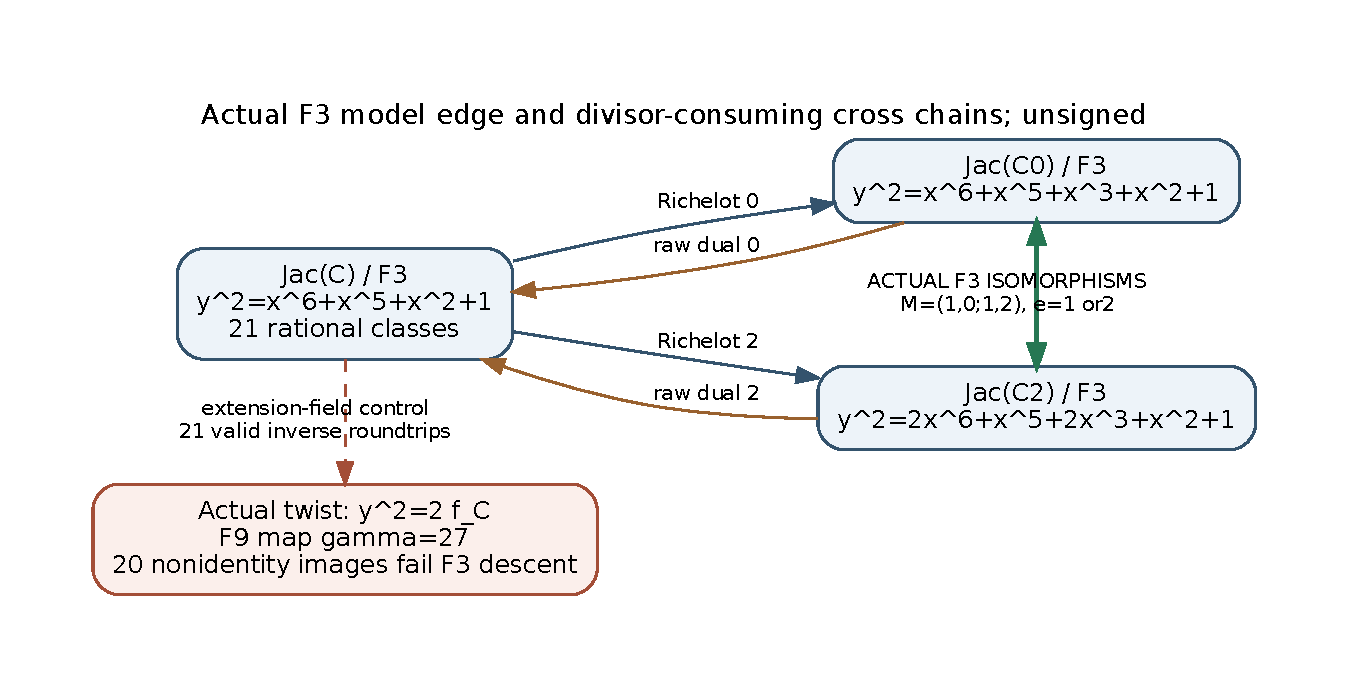
\includegraphics[width=0.97\linewidth]{models.pdf}\end{center}
\vspace{-3mm}
\begin{center}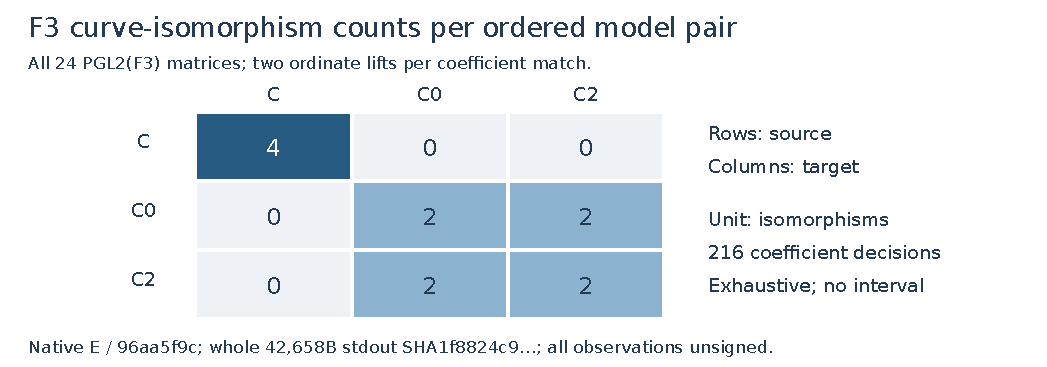
\includegraphics[width=0.88\linewidth]{isomorphisms.pdf}\end{center}
\vspace{-3mm}

\section{Every coefficient and every rational divisor}
All $24$ canonical $\operatorname{PGL}_2(\mathbb F_3)$ matrices on all
$9$ ordered model pairs give $216$ complete binary-sextic coefficient
decisions. The $12$ accepted curve maps each have $21$ distinct valid,
Frobenius-fixed divisor images, $441$ addition laws, $441$ scalar controls,
$24$ independent actual effective-pair comparisons and $21$ exact
weighted-inverse roundtrips. Frozen prior fixture data supplies the full
$63$ rational classes; the old constructor is not rerun. \uv

Both maps $C_0\leftrightarrow C_2$ use
\[
 M=\begin{pmatrix}1&0\\1&2\end{pmatrix},\qquad
 x'=\frac{x}{x+2},\qquad y'=\frac{e\,y}{(x+2)^3},\quad e=1,2.
\]
Actual homogeneous coordinates include denominator-zero points. The
map consumes a divisor, matrix, ordinate scale and charts; scalar labels
are used only by the reference driver. \uv

\newpage
{\Large\bfseries Finite actions, descent and reproduction}\par

\section{The actual cross-model loops}
Each route is an evaluated Richelot map, the model isomorphism and the
other raw dual, all consuming divisors. Both directions through the two
leaves give the same two finite action classes. \uv

\begin{center}\begin{tabular}{@{}llll@{}}
\toprule
Ordinate $e$ & Action on $J(C)(\mathbb F_3)$ & Order-$7$ action & Checks per route\\\midrule
$1$ & $16\pmod{21}$ & $+2\pmod7$ & $21$ images; $441$ additions\\
$2$ & $5\pmod{21}$ & $-2\pmod7$ & $21$ images; $441$ additions\\
\bottomrule\end{tabular}\end{center}

The source involution with matrix $M$ acts by $13$ for $e=1$ and $8$
for $e=2$ modulo $21$, with order-$3$/order-$7$ actions $(1,-1)$ and
$(-1,1)$. On this finite cohort the cross-loop action equals $-2$ times
that involution. These observations do not identify the algebraic maps
globally with $[16]$ or $[5]$. A generic functorial/kernel identity remains
a separate proof obligation. \uv

\section{A genuine extension-field positive and prime-field negative}
For $C_{\rm tw}:y^2=2f_C$, the identity matrix has coefficient scale $2$,
so neither $\mathbb F_3$ ordinate lift qualifies. The actual element
$\gamma=27$ in the native encoding satisfies
$\gamma^2=2$, $\gamma^9=\gamma$, $\gamma^3=-\gamma$.
The curve isomorphism over $\mathbb F_9$ gives all $21$ valid distinct
divisor images and restores all of them by the actual geometric inverse.
Their original Frobenius images equal their negatives: exactly $20$
nonidentity classes are not $\mathbb F_3$-fixed; identity is the positive
counterpart. No unconditional reject is used. \uv

\section{Complete first-failure flow and exact evidence}
\begin{center}\begin{tabular}{@{}L{0.18\linewidth}L{0.74\linewidth}@{}}
\toprule
Profile & Actual outcome retained\\\midrule
A & Formatting $1$; full $13{,}310$ B diagnostic.\\
B & Format $0$, strict compile $1$: unread inherited root field; $500$ B.\\
C & New root diagnostic formatting $1$; $511$ B.\\
D & Format/compile $0$, Clippy $1$: fixed chunk API; $703$ B.
Whole $4{,}783{,}760$ B ELF\texttt{ed5a4f19} remains unexecuted.\\
E & All seven phases $0$, source/copy/tool/immutable-ELF guards unchanged.
Full $42{,}658$ B stdout\texttt{1f8824c9}; all individual map and chain
outputs, coefficient catalog and twist controls retained.\\
\bottomrule\end{tabular}\end{center}

Rust1.99.1, shared Linux x86-64 development, $2$ GiB virtual memory,
$120$ seconds per phase, one worker. All $42$ frozen E inputs were
published and fully read back before first phases. Original A--D source
and diagnostics are immutable; no warning suppression or limit increase.
Whole E ELFs $4{,}783{,}872$ B, SHA prefix\texttt{578a2288}, remain
in original RAM custody pending approved-store/CI retention. \uv

\section{Proof map and next unit}
The native coefficient catalog and actual coordinate maps check this
finite construction. Written completeness uses the unique genus-$2$
hyperelliptic involution and the weighted projective form; the inverse
uses the canonical-adjugate cubic ordinate factor. Generic Mathlib and
the characteristic-$3$ identity-certificate bridge remain open.
The existing fixed $2^{61}-1$ certificate is not substituted. \uv

Next freeze the strongest cold reference, including source automorphisms,
then qualify the genuine nonhyperelliptic genus-$3$ source family. Costs,
actual Weil-$8$, product/extension routes and normal CI/merge gates remain
separate obligations. The earlier dual-only kernel result is scoped to
the fixed codomains; its historical dashed model edge is now evaluated. \uv

\begin{flushleft}\footnotesize
Full records: \path{model_isomorphism/first-E-native/models.stdout},
\path{model_isomorphism/ACTUAL_FIRST_E_RESULT.json} and
\path{model_isomorphism/CURRENT_RESULT_E.md}.
Primary sources read: Magma
\href{https://magma.maths.usyd.edu.au/magma/handbook/text/1626}{isomorphisms1626},
\href{https://magma.maths.usyd.edu.au/magma/handbook/text/1611}{twists1611}.
KB/Conductor unavailable, exact-source fallback, no novelty clearance. \uv
\quad\href{https://github.com/isogeny-labs/crypto/pull/5007}{PR5007}
\quad\href{https://github.com/isogeny-labs/crypto/issues/3904}{Queue3904}
\end{flushleft}
\end{document}
